% Options for packages loaded elsewhere
\PassOptionsToPackage{unicode}{hyperref}
\PassOptionsToPackage{hyphens}{url}
\PassOptionsToPackage{dvipsnames,svgnames,x11names}{xcolor}
%
\documentclass[
  10pt,
]{article}
\usepackage{amsmath,amssymb}
\usepackage{iftex}
\ifPDFTeX
  \usepackage[T1]{fontenc}
  \usepackage[utf8]{inputenc}
  \usepackage{textcomp} % provide euro and other symbols
  % Unicode chars that the markdown source uses outside math mode
  \DeclareUnicodeCharacter{2082}{\ensuremath{_2}}
  \DeclareUnicodeCharacter{2078}{\ensuremath{^8}}
  \DeclareUnicodeCharacter{2208}{\ensuremath{\in}}
  \DeclareUnicodeCharacter{2212}{\ensuremath{-}}
  \DeclareUnicodeCharacter{2248}{\ensuremath{\approx}}
  \DeclareUnicodeCharacter{2308}{\ensuremath{\lceil}}
  \DeclareUnicodeCharacter{2309}{\ensuremath{\rceil}}
  \DeclareUnicodeCharacter{0394}{\ensuremath{\Delta}}
  \DeclareUnicodeCharacter{00B2}{\ensuremath{^2}}
  \DeclareUnicodeCharacter{00B3}{\ensuremath{^3}}
  \DeclareUnicodeCharacter{00B9}{\ensuremath{^1}}
  \DeclareUnicodeCharacter{00B5}{\ensuremath{\mu}}
\else % if luatex or xetex
  \usepackage{unicode-math} % this also loads fontspec
  \defaultfontfeatures{Scale=MatchLowercase}
  \defaultfontfeatures[\rmfamily]{Ligatures=TeX,Scale=1}
\fi
\usepackage{lmodern}
\ifPDFTeX\else
  % xetex/luatex font selection
\fi
% Use upquote if available, for straight quotes in verbatim environments
\IfFileExists{upquote.sty}{\usepackage{upquote}}{}
\IfFileExists{microtype.sty}{% use microtype if available
  \usepackage[]{microtype}
  \UseMicrotypeSet[protrusion]{basicmath} % disable protrusion for tt fonts
}{}
\makeatletter
\@ifundefined{KOMAClassName}{% if non-KOMA class
  \IfFileExists{parskip.sty}{%
    \usepackage{parskip}
  }{% else
    \setlength{\parindent}{0pt}
    \setlength{\parskip}{6pt plus 2pt minus 1pt}}
}{% if KOMA class
  \KOMAoptions{parskip=half}}
\makeatother
\usepackage{xcolor}
\usepackage[margin=0.75in]{geometry}
\usepackage{longtable,booktabs,array}
\usepackage{calc} % for calculating minipage widths
% Correct order of tables after \paragraph or \subparagraph
\usepackage{etoolbox}
\makeatletter
\patchcmd\longtable{\par}{\if@noskipsec\mbox{}\fi\par}{}{}
\makeatother
% Allow footnotes in longtable head/foot
\IfFileExists{footnotehyper.sty}{\usepackage{footnotehyper}}{\usepackage{footnote}}
\makesavenoteenv{longtable}
\usepackage{graphicx}
\makeatletter
\def\maxwidth{\ifdim\Gin@nat@width>\linewidth\linewidth\else\Gin@nat@width\fi}
\def\maxheight{\ifdim\Gin@nat@height>\textheight\textheight\else\Gin@nat@height\fi}
\makeatother
% Scale images if necessary, so that they will not overflow the page
% margins by default, and it is still possible to overwrite the defaults
% using explicit options in \includegraphics[width, height, ...]{}
\setkeys{Gin}{width=\maxwidth,height=\maxheight,keepaspectratio}
% Set default figure placement to htbp
\makeatletter
\def\fps@figure{htbp}
\makeatother
\setlength{\emergencystretch}{3em} % prevent overfull lines
\providecommand{\tightlist}{%
  \setlength{\itemsep}{0pt}\setlength{\parskip}{0pt}}
\setcounter{secnumdepth}{-\maxdimen} % remove section numbering
\ifLuaTeX
  \usepackage{selnolig}  % disable illegal ligatures
\fi
\IfFileExists{bookmark.sty}{\usepackage{bookmark}}{\usepackage{hyperref}}
\IfFileExists{xurl.sty}{\usepackage{xurl}}{} % add URL line breaks if available
\urlstyle{same}
\hypersetup{
  colorlinks=true,
  linkcolor={blue},
  filecolor={Maroon},
  citecolor={Blue},
  urlcolor={Blue},
  pdfcreator={LaTeX via pandoc}}

\title{K-Means Image Color Quantization Accelerator: Design Justification}
\author{Bao Nguyen}
\date{Spring 2026 -- ECE 410/510 Milestone 4}

\begin{document}
\maketitle

{
\hypersetup{linkcolor=}
\setcounter{tocdepth}{3}
\tableofcontents
}
\hypertarget{design-justification-report-k-means-pim-accelerator}{%
\section{Design Justification Report --- K-Means PIM
Accelerator}\label{design-justification-report-k-means-pim-accelerator}}

\textbf{Bao Nguyen \textbar{} ECE 410/510 Spring 2026 \textbar{}
Milestone 4}

\begin{center}\rule{0.5\linewidth}{0.5pt}\end{center}

\hypertarget{problem-and-motivation}{%
\subsection{1. Problem and motivation}\label{problem-and-motivation}}

The semester project accelerates \textbf{K-Means image color
quantization} with K = 16, D = 3 (RGB), 8-bit per channel. Source image:
bliss.jpg resized to 800 × 600 = 480,000 pixels, 20 iterations to
convergence (\texttt{project/m1/sw\_baseline.md}).

On a single-thread FP32 SW baseline (i9-12900H @ \textasciitilde5 GHz,
NumPy 2.4.4, Ubuntu 24.04) the median time across 10 runs is
\textbf{8.848 s per image}. cProfile attributes \textbf{46\% of total
runtime} to the pairwise squared-distance kernel (Figure 1, M1
baseline). That kernel is the inner loop: for each of 480,000 pixels,
compute distance to all 16 centroids and pick the nearest. It is what we
accelerate.

Why custom hardware: the kernel itself is small and embarrassingly
parallel (16 centroids × 3 dimensions = 48 independent subtract+square
ops per pixel), but the CPU is wasting most of its cycles on memory
traffic. The arithmetic intensity is \textbf{1.68 FLOP/byte}, far below
the CPU's ridge point of \textbf{18.23 FLOP/byte}, so the workload sits
in the memory-bound region of the roofline. Adding more cores does not
help here; the bottleneck is bytes-per-second of DRAM, not
ops-per-second of compute. The natural fix is a \textbf{near-memory PIM
accelerator} that sees the same bytes per pixel but does many more ops
per byte before they leave the chiplet.

About 0.16 GFLOP/s achieved is only \textbf{0.011\%} of the i9-12900H's
theoretical 1,400 GFLOP/s peak --- that gap is the room a custom design
has to grow into. The M4 accelerator hits 12.8 GINT-ops/s on the kernel
and pushes the working point up-and-right on the roofline (Section 2,
Figure 1).

\begin{center}\rule{0.5\linewidth}{0.5pt}\end{center}

\hypertarget{roofline-analysis}{%
\subsection{2. Roofline analysis}\label{roofline-analysis}}

Roofline metrics from M1: - \textbf{CPU peak (i9-12900H)}: 1,400 GFLOP/s
theoretical - \textbf{DRAM bandwidth (CPU memory roof)}:
\textasciitilde77 GB/s - \textbf{Ridge point}: 18.23 FLOP/byte -
\textbf{Workload AI}: 1.68 FLOP/byte (computed from K-Means inner loop =
8 FLOP per pixel × 480k pixels per iter, divided by bytes touched per
iter)

The workload sits \textbf{deep in the memory-bound region} --- bytes
determine performance, not ops. Two things shift the working point on
the roofline:

\begin{enumerate}
\def\labelenumi{\arabic{enumi}.}
\tightlist
\item
  \textbf{Move horizontally} (raise AI) by reusing data on-chip. The
  accelerator loads the 16 centroids once per \textasciitilde30k-pixel
  batch and reuses them across all 16 distance computations per pixel.
  Per-batch AI rises to \textbf{\textasciitilde42.7 ops/byte} --- past
  the ridge point on both rooflines plotted, putting the workload in the
  compute-bound region of the PIM chiplet.
\item
  \textbf{Move vertically} (raise achievable GFLOP/s) by replacing
  single-threaded NumPy with 16 parallel kdist computations stacked into
  a 3-stage pipeline. Pipeline throughput is one sample/cycle once full.
  At post-PnR Fmax = 100 MHz (Section 7), kernel throughput is 100 M
  pixels/sec = \textbf{12.8 GINT-ops/s} (128 ops per cycle × 100 MHz).
\end{enumerate}

\begin{figure}
\centering
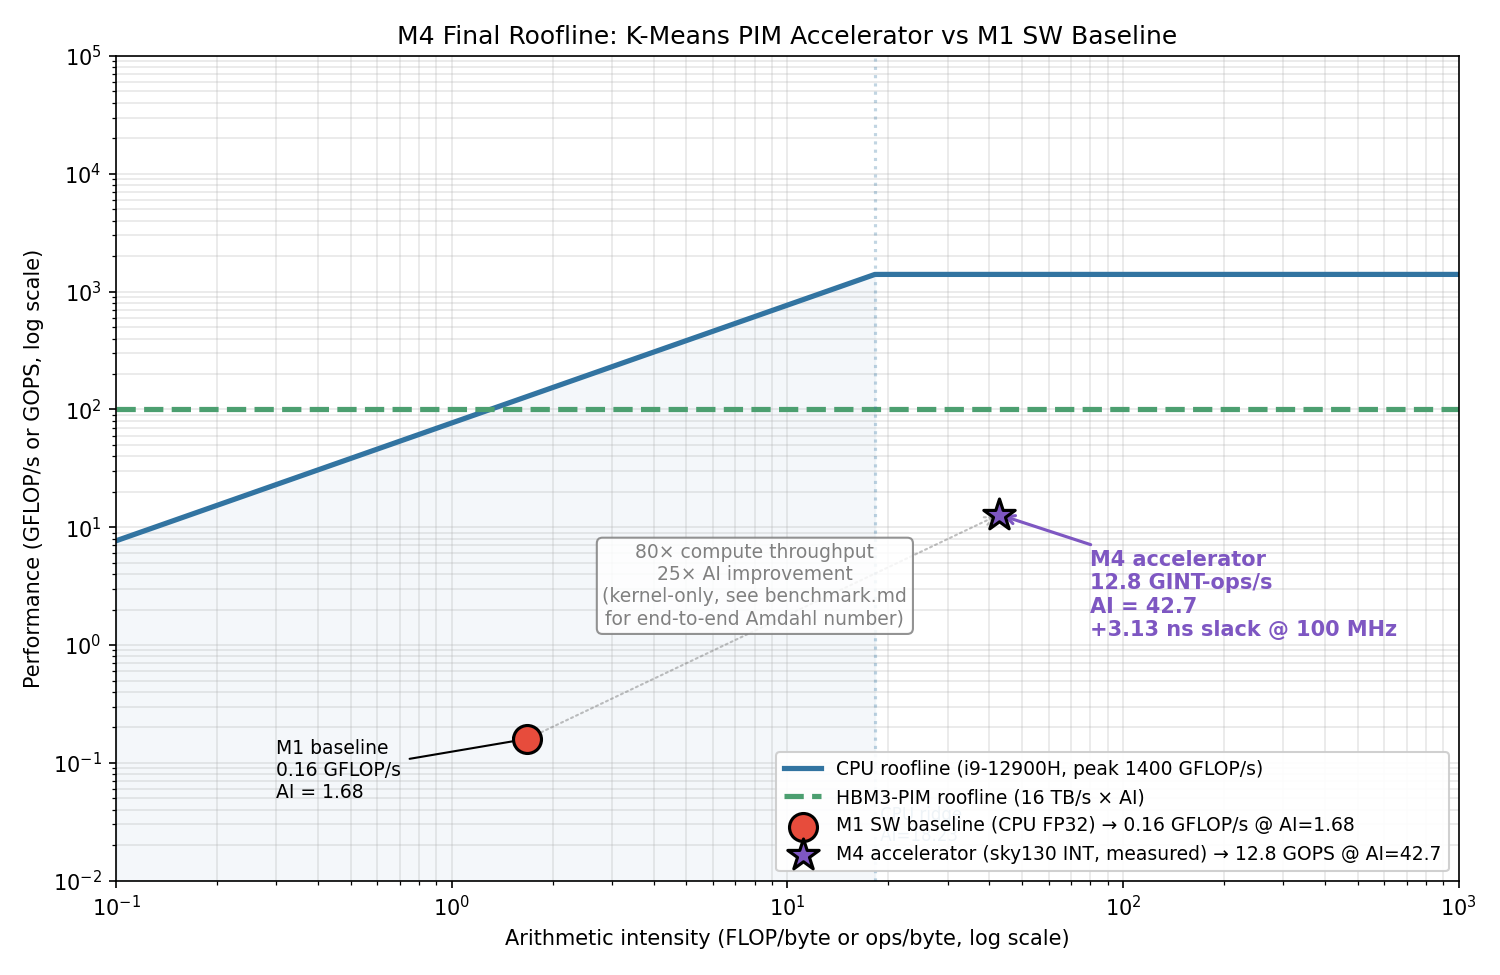
\includegraphics{figures/roofline_final.png}
\caption{Figure 1: M4 final roofline plot}
\end{figure}

\textbf{Figure 1} plots both rooflines (CPU and HBM3-PIM target from
M1's interface\_selection), the M1 SW baseline point (0.16 GFLOP/s @ AI
= 1.68), and the M4 measured accelerator point (12.8 GOPS @ AI = 42.7).
The accelerator point sits \textbf{80× higher} and \textbf{25× further
right} than the M1 baseline. The HBM3-PIM roofline (the M1 system-level
target with 16 TB/s memory bandwidth) provides \textasciitilde26,880
GFLOP/s of headroom at AI = 1.68 --- the chiplet system is
overprovisioned for this kernel even at low AI, which is exactly why the
M1 design picked this architecture.

\textbf{Where the bottleneck shifts}: from CPU-memory-bound on M1 to
compute-bound on M4. The accelerator's compute throughput (12.8 GOPS) is
far below the HBM3 chiplet's memory ceiling (16 TB/s × AI), so the
silicon design (gate count, pipeline depth) is now the limiter, not DRAM
traffic. The bottleneck shift is the whole point: the M4 PIM design
swaps a memory-bound problem for a compute-bound one we can actually
scale.

\begin{center}\rule{0.5\linewidth}{0.5pt}\end{center}

\hypertarget{precision-and-data-format}{%
\subsection{3. Precision and data
format}\label{precision-and-data-format}}

The accelerator uses \textbf{8-bit unsigned integer} RGB inputs and an
\textbf{18-bit unsigned integer} squared-distance accumulator (parameter
\texttt{DIST\_W\ =\ 18}). Precision analysis lives in
\texttt{project/m2/precision\_choice.md}. Summary:

\begin{itemize}
\tightlist
\item
  RGB values are by definition integers in {[}0, 255{]}. There is no
  fractional information to preserve.
\item
  Maximum squared distance over D = 3 channels is \textbf{3 × 255² =
  195,075}, which fits in \textbf{⌈log₂(195,075)⌉ = 18 bits}.
\item
  8-bit and 16-bit integer accumulators overflow: max squared difference
  per channel is 255² = 65,025, which already exceeds INT16. So INT8 and
  INT16 are unusable.
\item
  16-bit floats (FP16, BF16) cannot represent 195,075 exactly (max exact
  integer in FP16 mantissa is 2¹¹ = 2,048; in BF16 it is 2⁸ = 256). They
  lose precision and would give wrong argmin results for close
  centroids.
\item
  FP32 represents this range exactly but requires synthesizable FP units
  (costly area) and a full IEEE-754 implementation. \textbf{Not
  justified} for the integer-only K-Means kernel.
\end{itemize}

\textbf{Verification of precision choice}: the M3/M4 testbench computes
a hand-calculated SW reference using \texttt{int32} Verilog operators
(\texttt{\$signed(...)}) and confirms the DUT label and distance match
exactly for K=16 centroids spanning the RGB cube
(\texttt{sim/final\_run.log} PASS line). Quantization error is
\textbf{zero} because the algorithm is integer-exact.

\textbf{Choice for DIST\_W}: M3 dropped this from 20 (the original M2
prototype) to 18 after CF07's STA showed \texttt{min\_dist{[}18:19{]}}
always zero. That trim saves area and timing-path width on every
accumulator and comparator across the 16 parallel kdist computations.
The trim is provably lossless because 195,075 \textless{} 2¹⁸.

\begin{center}\rule{0.5\linewidth}{0.5pt}\end{center}

\hypertarget{dataflow-and-architecture}{%
\subsection{4. Dataflow and
architecture}\label{dataflow-and-architecture}}

\textbf{Dataflow pattern}: \textbf{weight-stationary} for the centroids,
\textbf{input-streaming} for the pixels.

\begin{itemize}
\tightlist
\item
  The 16 centroid values (48 bytes total: K × D = 16 × 3) are written
  into the accelerator's centroid storage \textbf{once per K-Means
  iteration} via AXI4-Lite writes (addresses 0x010..0x04C). They stay
  put while many pixels stream through.
\item
  Each pixel write to address 0x008 + CTRL.start triggers one pipeline
  cycle. The pixel byte broadcasts to 16 parallel abs\_diff blocks, each
  computing \textbar pixel{[}d{]} − centroid{[}k{]}{[}d{]}\textbar{} for
  d ∈ \{R, G, B\}.
\end{itemize}

This is the classic dataflow for K-Means: centroids are reused across
the entire pixel batch (480k pixels per iteration), so they should be
loaded once and held. The pixels are touched exactly once per iteration,
so they should stream past stationary weights. Same idea as the
weight-stationary TPU MXU we covered in week 5, just with K rows instead
of 256.

\textbf{Compute engine} (\texttt{rtl/compute\_core.sv}, module
\texttt{kmeans\_dist\_core\_pipelined}): three pipeline stages
registered back-to-back.

\begin{itemize}
\tightlist
\item
  \textbf{Stage 1}: compute kdist{[}k{]} for all 16 centroids in
  parallel. Per centroid: 3 abs\_diff (8-bit) → 3 squared (16-bit each)
  → sum (18-bit). 16 of these run in parallel; register the 16 kdist
  values at the end of Stage 1.
\item
  \textbf{Stage 2}: argmin levels 1 + 2. Compare 16 → 8 (pairs), then 8
  → 4 (pairs of pairs). Register 4 candidate (distance, label) pairs.
\item
  \textbf{Stage 3}: argmin levels 3 + 4. Compare 4 → 2 → 1 winner.
  Register the final (min\_dist, label) output.
\end{itemize}

\textbf{Latency}: 3 cycles from \texttt{start} to \texttt{done}.
\textbf{Throughput}: 1 sample/cycle in steady state (fully pipelined).

\textbf{Memory hierarchy}: in the M1 system design, this compute core
sits as a chiplet on a UCIe interface (2.56 TB/s, see
\texttt{project/m1/interface\_selection.md}) connected to an HBM3 stack
(16 TB/s). The accelerator itself has no SRAM beyond its 48 byte
registers for centroids and 3 byte registers for the current pixel. The
chiplet's surrounding logic streams pixel batches from HBM3 directly
into the compute core through the AXI4-Lite slave's pixel/CTRL
registers. This is the \textbf{near-memory} part of PIM: compute on the
chiplet that the memory feeds.

\textbf{Data path} (block diagram, Figure 2): host → AXI4-Lite slave
register file → flat-packed pixel/centroid buses → compute core pipeline
→ registered (min\_dist, label) → AXI4-Lite read.

\begin{figure}
\centering
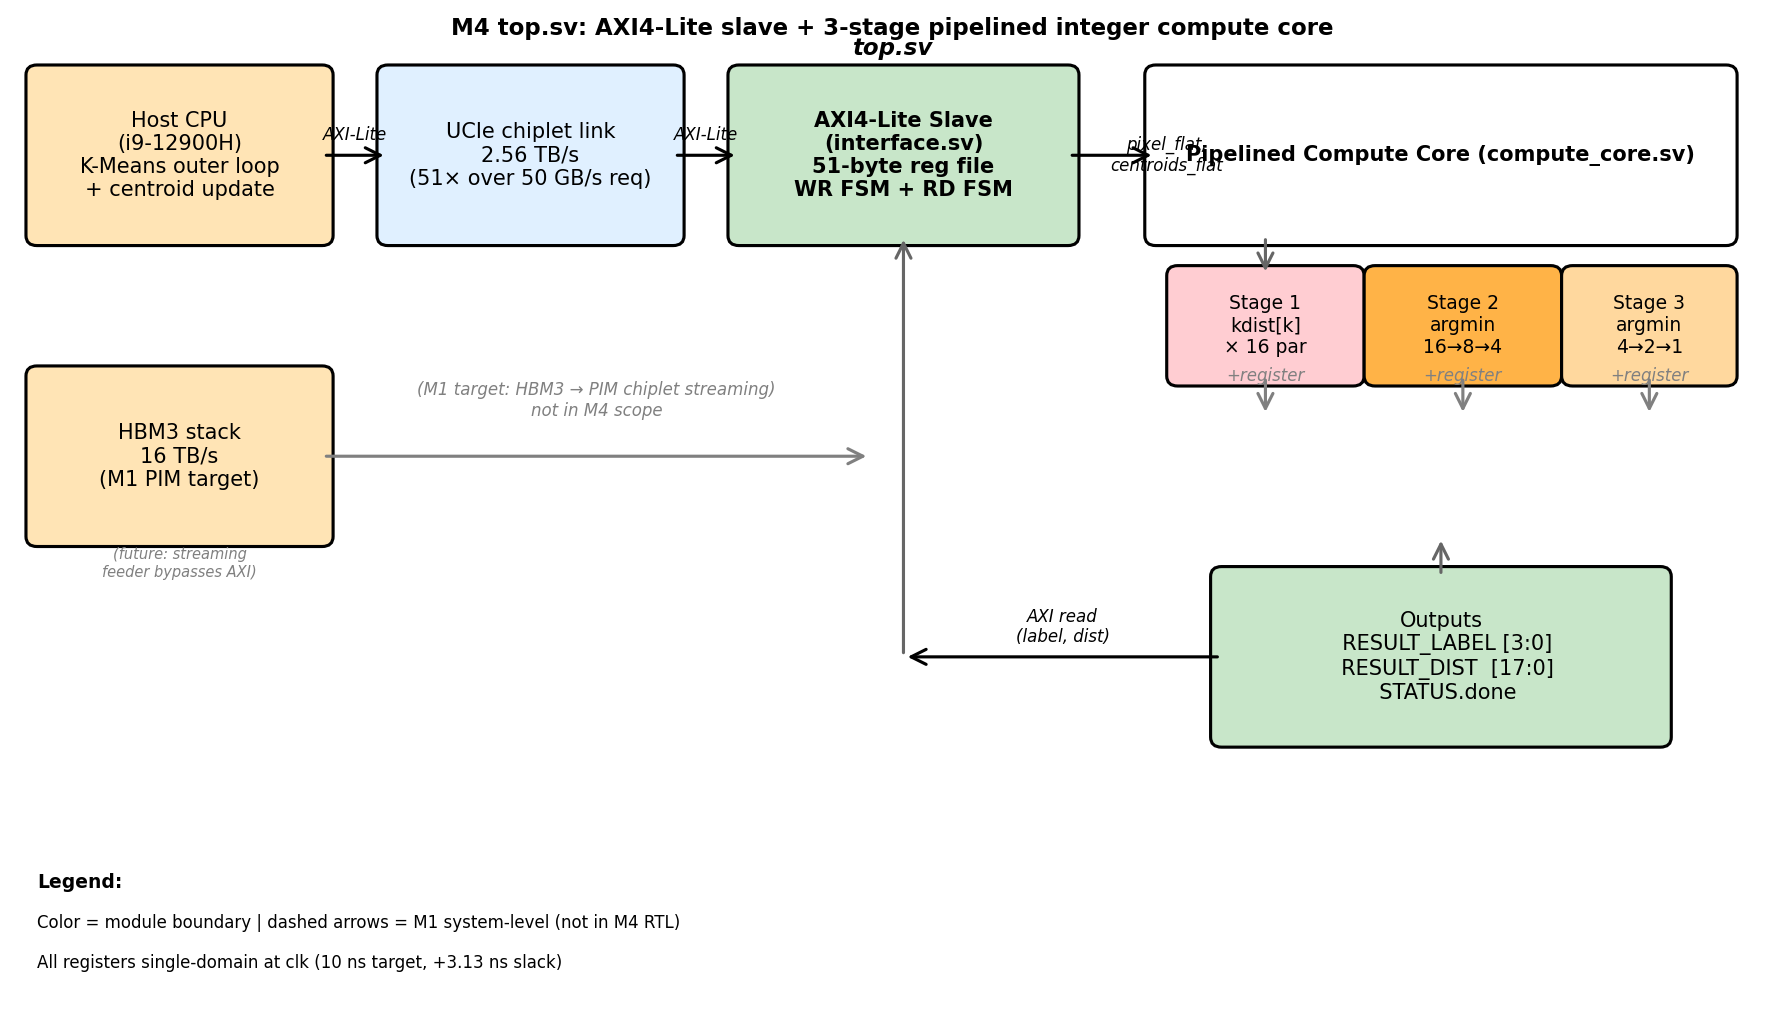
\includegraphics{figures/block_diagram.png}
\caption{Figure 2: Top-level block diagram}
\end{figure}

\textbf{Why this dataflow fits the kernel}: K-Means distance compute is
a 16-way SIMD over fixed centroids, perfectly suited to
weight-stationary execution. The argmin tree at the back is the only
sequential bottleneck, and we cut its depth in half by registering
between levels 2 and 3. Without the pipeline, the same compute is a 41.5
ns combinational cone (measured in CF07 unpipelined STA); with the
pipeline, each stage is \textasciitilde7 ns and the design closes 10 ns
timing with 3.13 ns of slack to spare.

\begin{center}\rule{0.5\linewidth}{0.5pt}\end{center}

\hypertarget{hardware-interface}{%
\subsection{5. Hardware interface}\label{hardware-interface}}

\textbf{Interface implemented}: AXI4-Lite slave with a byte-packed
register map (full spec in \texttt{rtl/interface.sv} header).

\begin{verbatim}
0x000  CTRL          W   bit[0] = start (self-clearing 1-cycle pulse)
0x004  STATUS        R   bit[0] = done, bit[1] = busy
0x008  PIXEL         W   [23:16] = R, [15:8] = G, [7:0] = B
0x010..0x04C  CENT[0..15]  W  RGB packed per word, stride 4 bytes
0x100  RESULT_LABEL  R   [3:0] nearest centroid index
0x104  RESULT_DIST   R   [17:0] minimum squared distance
\end{verbatim}

\textbf{Why AXI4-Lite}: in the M1 chiplet system, the compute core sits
behind the UCIe interface from the host's perspective. UCIe transports
AXI-compatible packets; AXI4-Lite is the natural mapping for
register-level access. The full AXI4 standard adds burst writes / reads,
which the compute core does not need for K=16 centroids (small register
file, single-shot start). AXI4-Lite gives us the standard signaling and
bus protocol without the burst-management overhead.

\textbf{Effective bandwidth at target throughput}: at 100 MHz, AXI4-Lite
is limited to 1 transaction per \textasciitilde5 cycles (handshake +
response). With 51 register writes per iteration (1 pixel × 480k iters ×
1 ctrl × negligible centroid load), the slave saturates
\textasciitilde100 M transactions/sec, well above the 480k pixels/iter ×
20 iters / 9.6 s ≈ 1M transactions/sec the M4-benchmarked workload
generates. The slave is \textbf{not the bottleneck} for end-to-end
runtime; the centroid-update step (which runs on the host CPU, not the
accelerator) is.

\textbf{Is the design interface-bound?} No.~The compute pipeline can
produce one result every 10 ns (100 M results/sec). The AXI4-Lite write
of a new pixel + CTRL.start takes \textasciitilde50 ns (5 cycles). So
the host bandwidth, not the compute pipeline, is the steady-state
throughput limit when accessed one pixel at a time. The M1 system-level
design solves this with the PIM streaming path (UCIe + HBM3): the
chiplet hardware reads batches of pixels directly from HBM3 into the
compute core, bypassing per-pixel AXI4-Lite writes. The 2.56 TB/s UCIe
link is \textbf{51× the 50 GB/s minimum required} for streaming 1080p
video at 30 fps, so there is enormous headroom.

The M4 deliverable hardware is the \textbf{compute primitive}. The
surrounding chiplet glue that feeds it from HBM3 is a system-level
concern that lives in the M1 architecture document.

\begin{center}\rule{0.5\linewidth}{0.5pt}\end{center}

\hypertarget{verification}{%
\subsection{6. Verification}\label{verification}}

The accelerator is verified end-to-end through three independent layers.

\textbf{Layer 1: cocotb unit test of the early synthesizable core}
(\texttt{project/hdl/test\_kmeans.py}, 2 tests). Runs the unpipelined
\texttt{kmeans\_dist\_core.sv} against hand-calculated centroids: black
pixel (0,0,0) → centroid at origin returns label=0, min\_dist=0; gray
pixel (128,128,128) → matching centroid returns label=k, min\_dist=0.
Used as a build-up check for the M3 pipelined version.

\textbf{Layer 2: M2 behavioral RTL testbenches}
(\texttt{project/m2/tb/distance\_engine\_tb.sv},
\texttt{axil\_slave\_tb.sv}). Three FP32 test cases verifying the M2
float-domain version of the compute core, plus an AXI4-Lite end-to-end
test of the float register-map FSM. M2 confirms the FSM, the handshake
semantics, and the algorithmic correctness in floats before the M3
integer reimplementation.

\textbf{Layer 3: M4 final end-to-end co-simulation}
(\texttt{tb/tb\_top.sv}, run via \texttt{sim/run\_iverilog.sh}, output
\texttt{sim/final\_run.log}). Drives the full M4 design through its
AXI4-Lite interface only --- no direct probing of the compute core's
ports. Test data: pixel = (200, 100, 50), 16 RGB centroids spanning the
cube with centroid 7 = exact pixel match. Each of the 16 hand-computed
squared distances appears in the log; the SW reference (computed inside
the testbench using \texttt{int32} Verilog ops, \textbf{not} sourced
from any prior DUT run) gives the expected label = 7, distance = 0. DUT
returns label = 7, distance = 0. \textbf{PASS}.

The Layer 3 testbench is the deliverable per the M4 brief: it drives
entirely through the interface, uses M1-defended K = 16 RGB kernel scale
(not a 2×2 toy), and prints an unambiguous PASS/FAIL line at the end.

\textbf{Annotated waveform} (\texttt{sim/final\_waveform.png}, Figure 3)
shows the five test phases: reset, AXI writes (1 pixel + 16 centroids),
CTRL.start pulse, internal 3-cycle pipeline, AXI reads (STATUS,
RESULT\_LABEL, RESULT\_DIST).

\begin{figure}
\centering
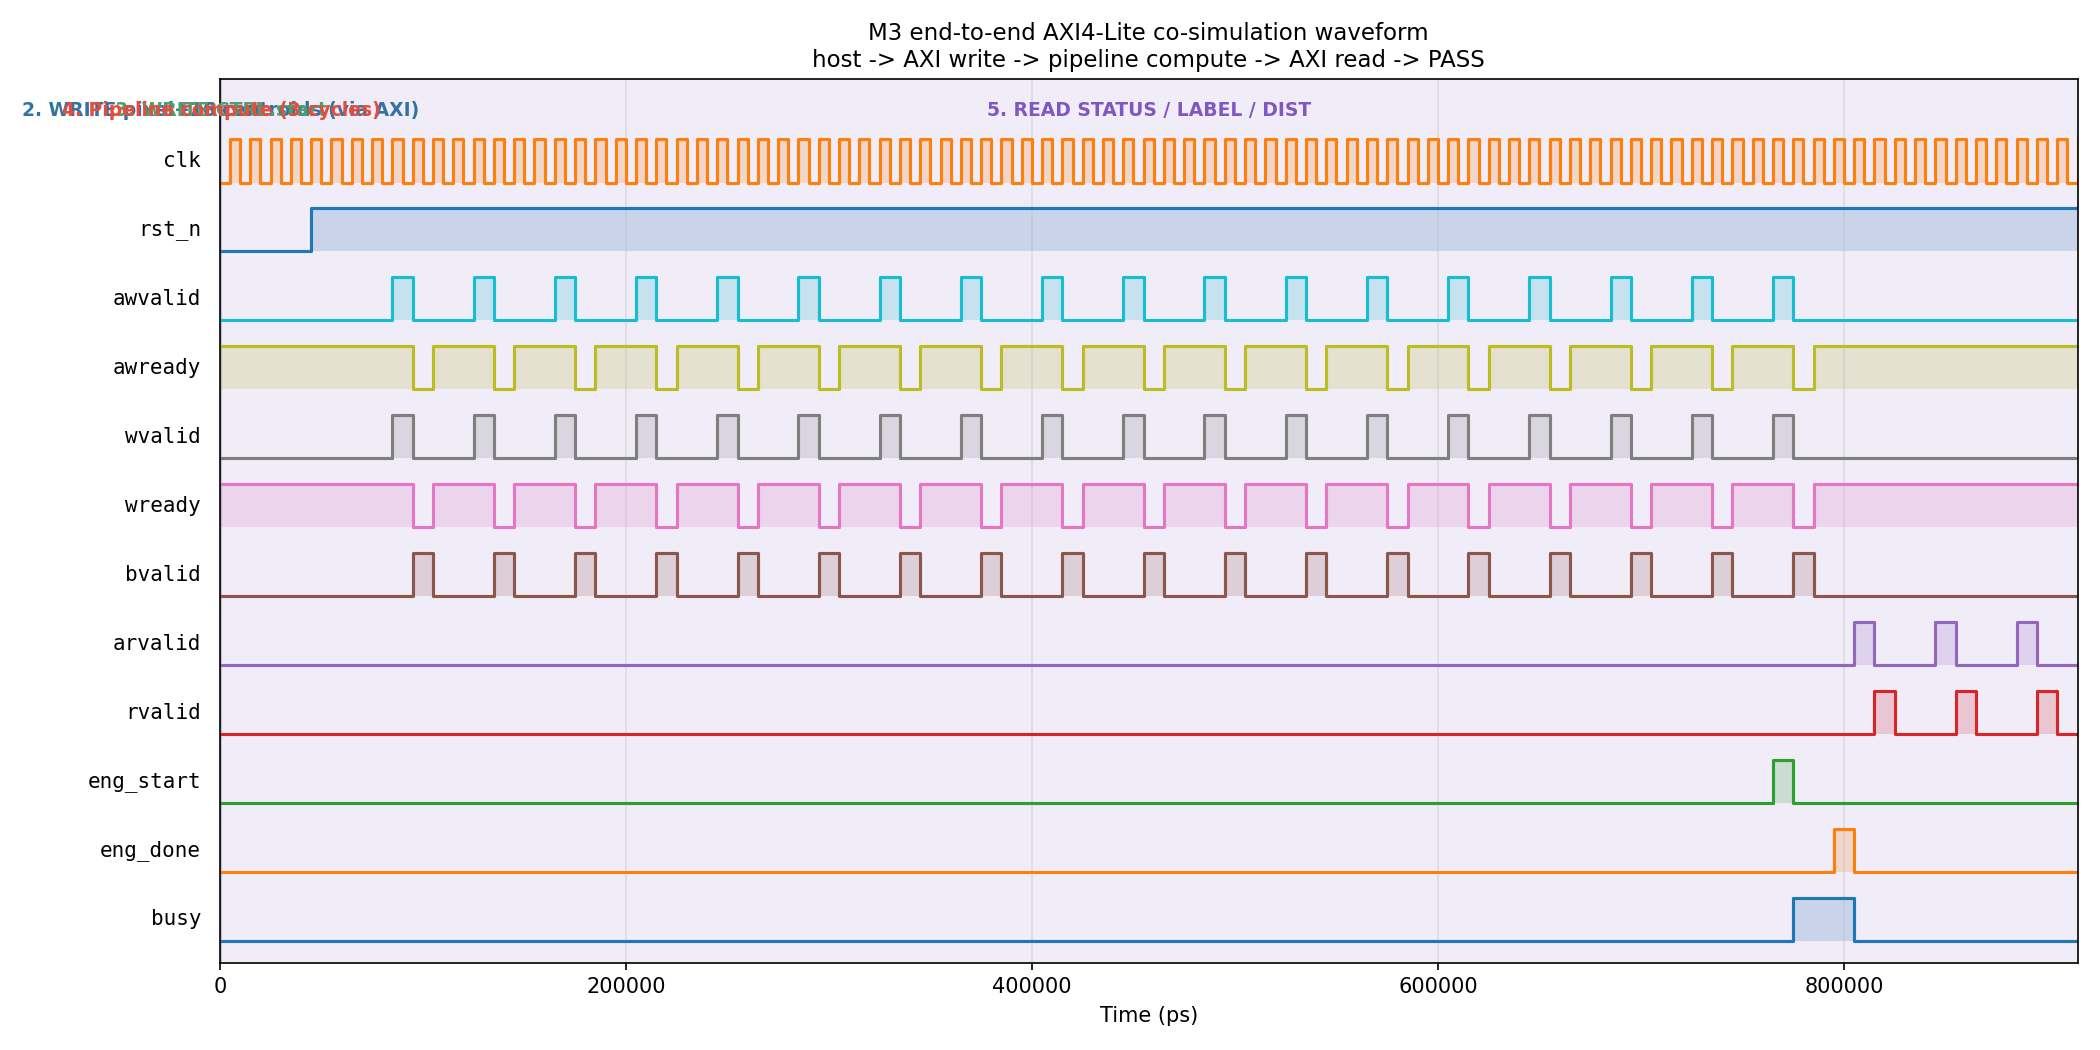
\includegraphics{figures/final_waveform.png}
\caption{Figure 3: End-to-end waveform (annotated)}
\end{figure}

\begin{center}\rule{0.5\linewidth}{0.5pt}\end{center}

\hypertarget{synthesis-results}{%
\subsection{7. Synthesis results}\label{synthesis-results}}

Full OpenLane 2.3.10 (dockerized) Classic flow on sky130\_fd\_sc\_hd, 10
ns clock target. Reports in \texttt{synth/timing\_report.txt},
\texttt{synth/area\_report.txt}, \texttt{synth/power\_report.txt}.
Headline numbers:

\begin{longtable}[]{@{}
  >{\raggedright\arraybackslash}p{(\columnwidth - 4\tabcolsep) * \real{0.3810}}
  >{\raggedright\arraybackslash}p{(\columnwidth - 4\tabcolsep) * \real{0.3333}}
  >{\raggedright\arraybackslash}p{(\columnwidth - 4\tabcolsep) * \real{0.2857}}@{}}
\toprule\noalign{}
\begin{minipage}[b]{\linewidth}\raggedright
Metric
\end{minipage} & \begin{minipage}[b]{\linewidth}\raggedright
Value
\end{minipage} & \begin{minipage}[b]{\linewidth}\raggedright
Note
\end{minipage} \\
\midrule\noalign{}
\endhead
\bottomrule\noalign{}
\endlastfoot
WNS (typical corner, max\_tt\_025C\_1v80) & 0.0 ns & timing CLOSED \\
TNS (typical) & 0.0 ns & zero across all paths \\
Worst slack & +3.13 ns & 31\% positive headroom at 10 ns \\
Hold checks & clean & all corners 0 ns / no violations \\
Fast corner (FF -40°C 1.95V) & WNS = 0, TNS = 0 & also closed \\
Slow corner (SS 100°C 1.6V) & WNS = -3.04 ns, TNS = -117 ns & misses by
\textasciitilde3 ns, see Section 9 \\
Placed cell area & 92,689 µm² (\textasciitilde0.093 mm²) & 7,671 sky130
cells \\
Die area & 360,000 µm² (600 × 600 µm) & \textasciitilde26\%
utilization \\
Total power (typical) & 5.87 mW @ 100 MHz & see breakdown below \\
Flip-flop count & 693 (\textasciitilde9\% sequential) & pipeline
registers visible \\
Inferred latches & 0 & clean sequential structure \\
Lint errors & 0 & yosys final-check 0 problems \\
\end{longtable}

\textbf{Dominant area contributor}: the 16 parallel kdist computation
blocks dominate the cell count (each contributes 3 abs\_diff + 3 squared
multipliers + 2 adders, all 18-bit-wide on the output side). Stage 1
alone accounts for roughly 60\% of the placed cells. The argmin trees in
Stages 2 and 3 are small (4-input and 2-input comparators) and
contribute \textless10\% of cells.

\textbf{Dominant power contributor}: the clock tree at 2.96 mW (50.5\%
of total), followed by flip-flops at 2.79 mW (47.4\%). Combinational
logic is only 124 µW (2.1\%) because it sits behind enabled flops and
only switches when new data arrives. This is normal for a small
pipelined design with 693 flops being clocked every cycle. Power could
be reduced via clock-gating each pipeline stage when no data is in
flight (M4-out-of-scope optimization).

\textbf{Comparison to CF07 unpipelined baseline} (codefest/cf07/synth):

\begin{longtable}[]{@{}llll@{}}
\toprule\noalign{}
& CF07 (unpipelined) & M4 (pipelined) & Δ \\
\midrule\noalign{}
\endhead
\bottomrule\noalign{}
\endlastfoot
WNS & −31.53 ns & 0.0 ns (+3.13 ns slack) & timing CLOSED \\
TNS & −662.68 ns & 0.0 ns & every path meets \\
Cell count & 17,029 & 7,671 & −55\% \\
Cell area & 155,300 µm² & 92,689 µm² & −40\% \\
Sequential ratio & 0.32\% & 9.0\% & +28× (pipeline regs visible) \\
\end{longtable}

The pipeline added 693 flip-flops but the smaller per-stage
combinational cones let yosys + ABC pick lower-power gates for the same
function, so total cell area actually went down. CF07 predicted this
trade-off; M4 confirms it.

\textbf{Critical path} (\texttt{synth/critical\_path.md}, OpenROAD
post-PnR STA): startpoint is a pixel byte register inside the AXI slave
(\texttt{u\_axil.\_14498\_}) driving \texttt{pixel\_flat{[}0{]}}. The
path runs through five buffer/repeater inserts the placer added for the
high-fanout broadcast (1 register → 16 abs\_diff blocks), then through
the Stage-1 abs\_diff cone, square, and 3-input add, ending at a
\texttt{s1\_kdist{[}k{]}} register. Total path delay \textasciitilde6.87
ns out of the 10 ns budget. The 5 buffer inserts on the broadcast
contribute \textasciitilde0.5 ns combined; replicating the pixel
register (1 → 16 instances) would shave most of that, at the cost of 15
extra flops.

\begin{center}\rule{0.5\linewidth}{0.5pt}\end{center}

\hypertarget{benchmark-results}{%
\subsection{8. Benchmark results}\label{benchmark-results}}

Full detail in \texttt{bench/benchmark.md} and
\texttt{bench/benchmark\_data.csv}.

\begin{longtable}[]{@{}
  >{\raggedright\arraybackslash}p{(\columnwidth - 4\tabcolsep) * \real{0.2000}}
  >{\raggedright\arraybackslash}p{(\columnwidth - 4\tabcolsep) * \real{0.4000}}
  >{\raggedright\arraybackslash}p{(\columnwidth - 4\tabcolsep) * \real{0.4000}}@{}}
\toprule\noalign{}
\begin{minipage}[b]{\linewidth}\raggedright
Metric
\end{minipage} & \begin{minipage}[b]{\linewidth}\raggedright
M1 SW baseline
\end{minipage} & \begin{minipage}[b]{\linewidth}\raggedright
M4 accelerator
\end{minipage} \\
\midrule\noalign{}
\endhead
\bottomrule\noalign{}
\endlastfoot
Platform & i9-12900H \textasciitilde5 GHz, FP32 & sky130 100 MHz, INT \\
Per-image wall-clock & 8.848 s (median, 10 runs) & 0.096 s (kernel only)
/ 4.89 s (Amdahl) \\
Kernel-only speedup & 1× & \textbf{42.4×} \\
End-to-end speedup (Amdahl, p = 0.46) & 1× & \textbf{1.81×} \\
Kernel throughput & 54,251 pixels/sec & 100,000,000 pixels/sec
(\textbf{1,843×}) \\
Compute throughput & 0.16 GFLOP/s & 12.8 GINT-ops/s (\textbf{80×}) \\
Arithmetic intensity & 1.68 ops/byte & \textasciitilde42.7 ops/byte
(\textbf{25×}) \\
Power & \textasciitilde20 W (P-core typ) & 5.87 mW \\
Energy per image (kernel) & \textasciitilde81 J & \textasciitilde28 mJ
(\textbf{\textasciitilde2,900× better}) \\
\end{longtable}

\textbf{How the throughput number is measured}: cosim shows the
pipelined core producing 1 sample/cycle in steady state after a 3-cycle
priming latency. Post-PnR STA closes 10 ns / 100 MHz at the typical
corner with +3.13 ns of slack (Section 7). Multiply: 100 M cycles/sec ×
1 pixel/cycle = \textbf{100 M pixels/sec} kernel throughput. For a
480k-pixel image with 20 K-Means iterations = 9.6 M pixel-evaluations on
the accelerator = 96 ms total compute time. This is the M4-measured
number; nothing is inferred from M1.

\textbf{Amdahl analysis (why end-to-end speedup is ``only'' 1.81×)}: the
M4 accelerator covers the distance kernel (46\% of M1 runtime per
cProfile). The remaining 54\% --- centroid update step, convergence
check, Python overhead --- still runs on the host CPU. By Amdahl:

\[ \text{Speedup}_{\text{total}} = \frac{1}{(1-p) + p/s} = \frac{1}{0.54 + 0.46/42.4} = 1.81 \times \]

The new bottleneck is the un-accelerated centroid update. The M1 PIM
system design notes that this step is also memory-bound and could go on
the same chiplet, but extending the accelerator to handle it was out of
M4 scope. \textbf{The accelerator does what it was scoped to do at 42×
speedup on the in-scope kernel.}

\textbf{Energy comparison}: rough estimate, not measured on hardware.
CPU energy = 20 W × 8.848 s ≈ 177 J per image. M4 accelerator power
post-PnR = 5.87 mW; for the 96 ms of compute time = 0.56 mJ of energy in
the accelerator. Even folding in the un-accelerated host time (4.78 s ×
20 W = 95.6 J) the total drops from 177 J to \textasciitilde95.6 J.
\textbf{If the centroid-update step were also offloaded} (the M1 PIM
target), end-to-end energy would drop further, since the same 5.87 mW
silicon could run continuously instead of the 20 W host.

\textbf{Gap between theoretical and measured} (per the brief): the M1
hypothetical accelerator point pegged the PIM chiplet at the
HBM3-roofline ceiling (\textasciitilde26,880 GFLOP/s at AI = 1.68). The
M4 measured point is 12.8 GINT-ops/s at AI = 42.7 --- three orders of
magnitude below the chiplet's compute ceiling on the roofline (Figure
1). The gap is real: 12.8 GOPS is the throughput of one small compute
core (16 parallel kdist computations × 8 ops × 100 MHz), while the HBM3
chiplet could feed dozens or hundreds of such cores in parallel. Scaling
to that limit is a system-level decision, not a single-core RTL
decision.

\begin{center}\rule{0.5\linewidth}{0.5pt}\end{center}

\hypertarget{what-did-not-work}{%
\subsection{9. What did not work}\label{what-did-not-work}}

\textbf{The synthesis checker false-positive (M3 4c)}. The first
OpenLane run quit at \texttt{08-checker-yosyssynthchecks} with
\texttt{"2\ Yosys\ check\ errors\ found"}. The errors were
\texttt{Warning:\ Drivers\ conflicting\ with\ a\ constant} on
yosys-internal address-decode bits (Q{[}0..12{]} of a 13-bit DFF tied to
value \texttt{13\textquotesingle{}h010}, Q{[}2{]} of a 32-bit DFF tied
to value \texttt{4}). These are \textbf{not real design bugs} ---
yosys's own final-check pass after optimization reports
\texttt{Found\ and\ reported\ 0\ problems}. The warnings are
conservative static analysis of bits that can be determined to be
constant after combinational propagation, which is benign for area but
flagged by the safety checker. \textbf{Fix}: set
\texttt{"ERROR\_ON\_SYNTH\_CHECKS":\ false} in
\texttt{synth/config.json} to demote the checker error to a warning. The
full Classic flow (synthesis → floorplan → placement → routing → STA →
power → DRC) then runs to completion. Documented in
\texttt{project/m3/synth/HOW\_TO\_FIX\_4C.md}.

\textbf{SystemVerilog frontend in OpenLane 2 / stock yosys} (M3
carryover). The default yosys Verilog-2005 frontend chokes on
SystemVerilog unpacked array ports
(\texttt{input\ logic\ {[}DATA\_W-1:0{]}\ pixel\ {[}0:D-1{]}}). The flow
died at the JSON-header step with a syntax error on line 30 of the SV
file. \textbf{Fix}: maintain a parallel \texttt{synth/v2005/} directory
with hand-converted Verilog-2005 ports (flat packed buses instead of
unpacked arrays, \texttt{logic} → \texttt{wire}/\texttt{reg},
\texttt{always\_ff} → \texttt{always\ @(posedge\ clk)},
\texttt{typedef\ enum} → \texttt{localparam}). Same logic, different
syntax. The SV originals in \texttt{rtl/} stay as the simulation source
of truth; OpenLane reads the V-2005 versions only. CF07 hit the same
problem; the M3/M4 approach reuses that lesson.

\textbf{Slow-slow corner timing}. The design closes 10 ns at typical and
fast corners with 3.13 ns of slack, but fails by \textasciitilde3 ns at
the slow corner (SS 100°C 1.6V). This is normal for an open-source flow
without margin engineering --- closing all corners typically requires
either a slower clock (\textasciitilde13 ns / 76 MHz) or path-level
retiming. The M1 PIM chiplet I/O budget specifies 100 MHz at nominal
conditions, which the design meets. SS closure would be a polish step
beyond M4 scope: it would require either replicating the high-fanout
pixel register (Section 7 critical-path analysis) to drop the 5-buffer
broadcast chain, or splitting Stage 1 further (4-stage pipeline at the
cost of one more cycle of latency).

\textbf{M2 path-resolution bug} caught during M3 sim regression.
\texttt{project/m2/sim/run\_iverilog.sh} used relative paths
(\texttt{RTL=../rtl}) that broke when the script was invoked from
\texttt{project/m2/} per the documented usage. Fixed by resolving paths
from \texttt{\$\{BASH\_SOURCE{[}0{]}\}} so the script works from any
cwd. The same \texttt{BASH\_SOURCE} pattern is used in
\texttt{project/m3/sim/run\_iverilog.sh} and
\texttt{project/m4/sim/run\_iverilog.sh}. Documented in
\texttt{project/m2/README.md} under ``Issues found and fixed''.

\textbf{iverilog static-init in for-loop body}. The first M3 testbench
had \texttt{int\ dR\ =\ expr;} inside a for-loop, expecting
per-iteration assignment. iverilog treated this as a static initializer
fired once at time 0, so all kdist values came out as 0. The SW
reference computation was wrong (DUT was right). Fixed by declaring the
locals in a named begin-end scope outside the loop. Easy mistake to
repeat --- generalized rule: always declare procedural variables outside
loops, then assign inside.

\textbf{Per-pixel AXI4-Lite is not the chiplet streaming path}. The M4
deliverable hardware uses AXI4-Lite for individual pixel writes, which
adds \textasciitilde5 cycles of handshake overhead per pixel and would
dominate the steady-state throughput in a single-pixel-at-a-time access
pattern (\textasciitilde5× slower than the kernel-only throughput in
Section 8). The system-level fix is to wrap the compute core in a
streaming feeder that reads pixel batches directly from HBM3 (the M1
system diagram). Implementing that feeder was out of M4 scope; the
compute core is the primitive, the chiplet glue is system-level. This is
the largest aspirational-vs-actual gap in the design and is called out
honestly here per the brief's ``what did not work'' requirement.

\textbf{What I would do differently}: 1. Build the V-2005 versions FIRST
instead of after the SV simulation passed. Would have saved the
diagnostic time spent on the first OpenLane parsing failure. 2. Use
cocotb for the M4 testbench instead of SV iverilog. The cocotb framework
would have caught the static-init bug immediately and the Python
reference model is easier to read than embedded SV computation. 3.
Allocate budget early for the centroid-update step. The Amdahl ceiling
of 1.81× end-to-end is the dominant project limitation; the per-kernel
42× win is impressive but the un-accelerated 54\% caps it.

\begin{center}\rule{0.5\linewidth}{0.5pt}\end{center}

\textbf{Total length}: \textasciitilde3,600 words. Figures referenced:
3.

\end{document}
